\documentclass[english]{beamer} %,handout
\usepackage{amsmath}
\usepackage{graphicx,subfig}
\usepackage{booktabs}
\usepackage{multirow}

\makeatletter

\usepackage{listings}
\usetheme{Boadilla}
\graphicspath{{../figure/}}

\setbeamercovered{transparent}

\usecolortheme{purdue}

\usepackage{babel}

\begin{document}

\title[HSM \& RNN]{Hierarchical Softmax for Recurrent Language Model}

\author{Nan Jiang$^{\dag}$, Wenge Rong$^{\dag}$, Min Gao$^{\S}$, Yikang Shen$^{\sharp}$ and Zhang Xiong$^{\dag}$}


\institute[univerisity]{
       $^{\dag}$ School of Computer Science and Engineering, Beihang University, China  \\
       $^{\S}$ School of Software Engineering, Chongqing University, China \\
       $^{\sharp}$ Montr\'eal Institute for Learning Algorithms, Universt\'e de Montr\'eal, Canada\\
}

\begin{frame}
  \titlepage
\end{frame}

\newcommand{\Gaussian}{\rput(0,-0.35){\psset{yunit=0.8cm,xunit=0.3}
     \psGauss[linecolor=red, linewidth=0.8pt, sigma=0.5]{-1.5}{1.5}}}
\def\dedge{\ncline[linestyle=dashed]}
\def\omitnode{\Tr*[edge=\dedge]{}}



\begin{frame}[<+->]{Outlines}
\begin{itemize}
\item Knowledge on recurrent language model;
\item Review on historical optimization methods;
\item Introduce our work on hierarchical softmax;
\item Experimental results.
\end{itemize}
%\begin{uncoverenv}%{}
%<3->
%\begin{exampleblock}
%{Two processes}
%\begin{itemize}
%\item $\left[\begin{array}{cc}
%p_{00} & p_{01}\\
%p_{10} & p_{11}\end{array}\right]$
%\item $\sum_{i}p_{ji}=1$
%\item  $\left[\begin{array}{cc}
%p_{00} & p_{01}\\
%p_{10} & p_{11}\end{array}\right]\left[\begin{array}{c}
%N_{0}(t)\\
%N_{1}(t)\end{array}\right]=\left[\begin{array}{c}
%N_{0}(t+1)\\
%N_{1}(t+1)\end{array}\right]$
%\end{itemize}
%\end{exampleblock}
%\end{uncoverenv}%{}
\end{frame}

\begin{frame}[<+->]{Recurrent Neural Language Model}

  \begin{center}
    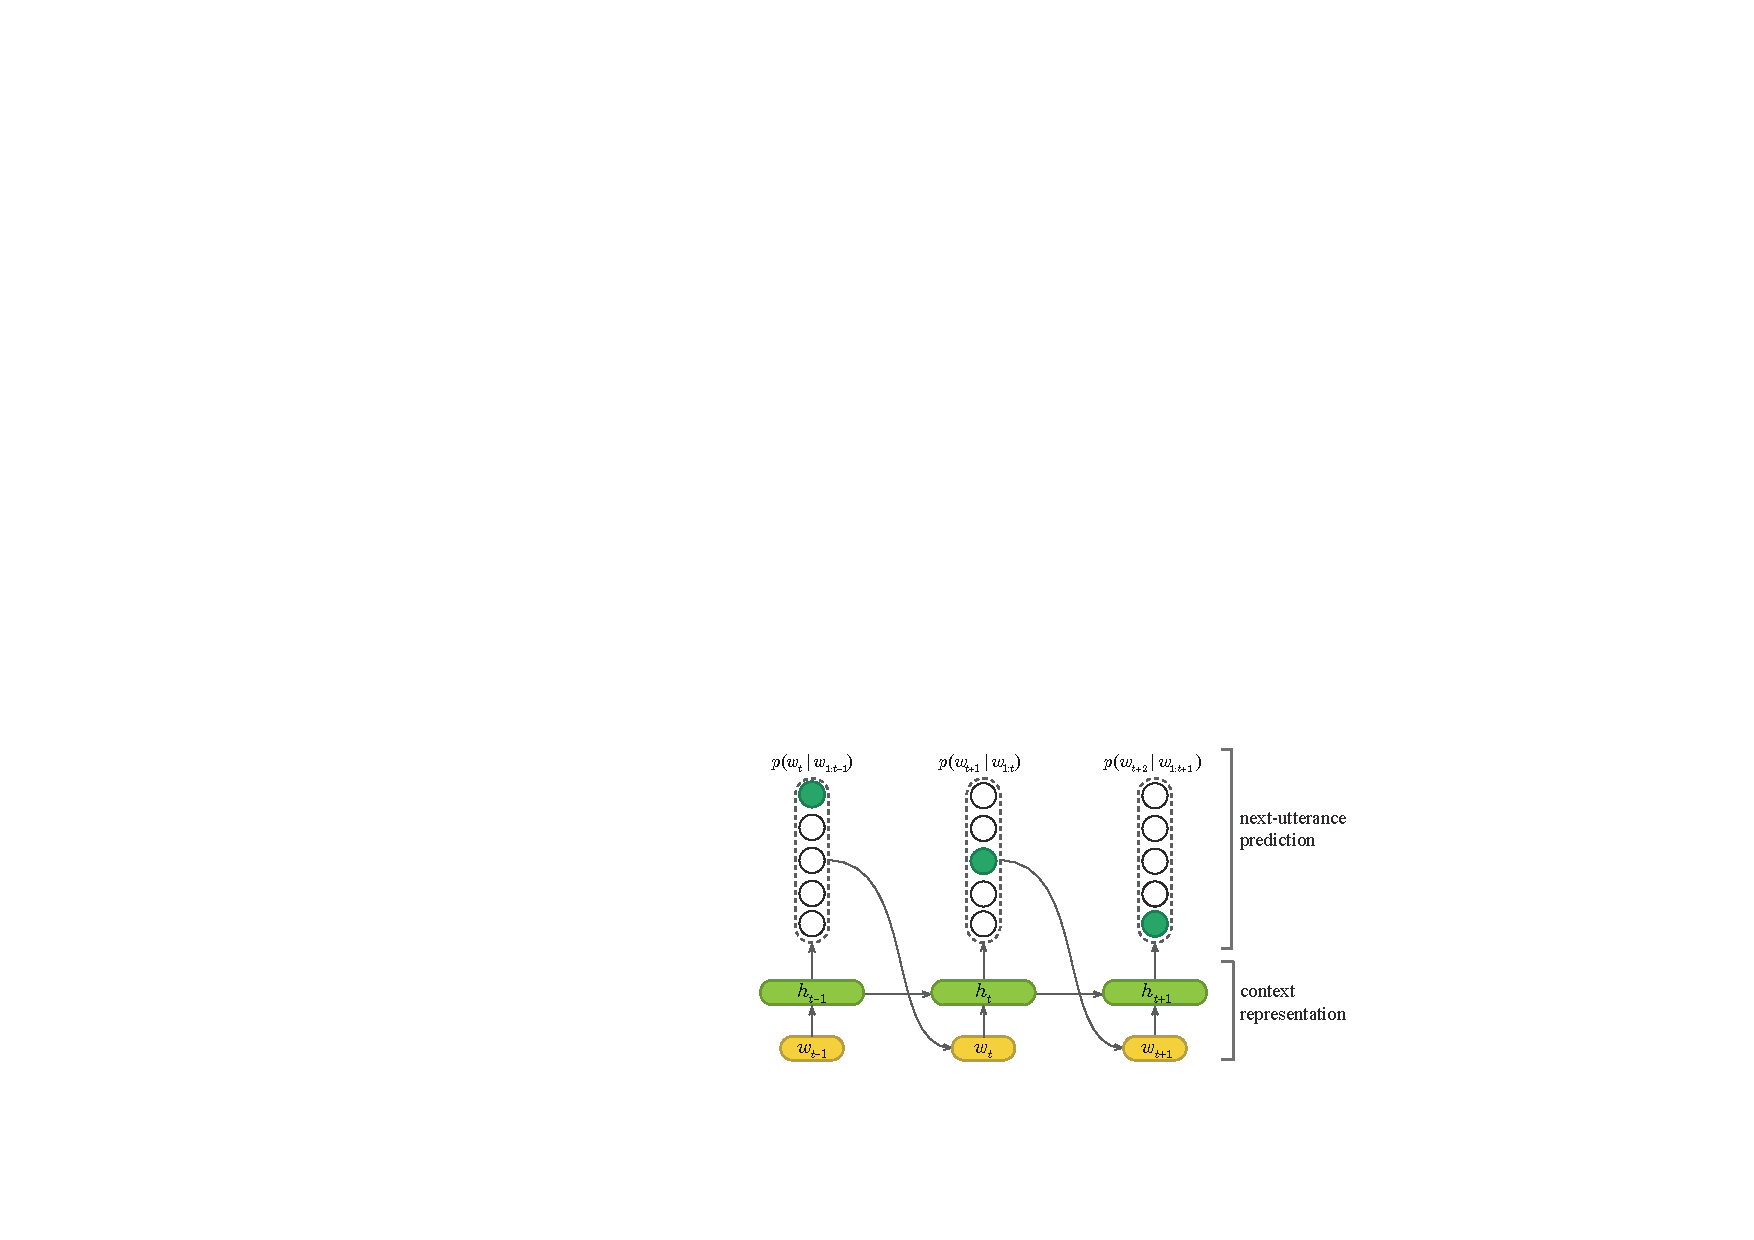
\includegraphics[scale=0.8]{lm}
  \end{center}

  \begin{equation}
 \log p(w_1,\cdots, w_T ) = \sum_{t=1}^T \log p(w_t | w_{1:t-1}),
\end{equation}
Trade off between speed and accuracy.
\end{frame}

\begin{frame}[<+->]{Datasets}
Dataset involved in this research.
\begin{center}
    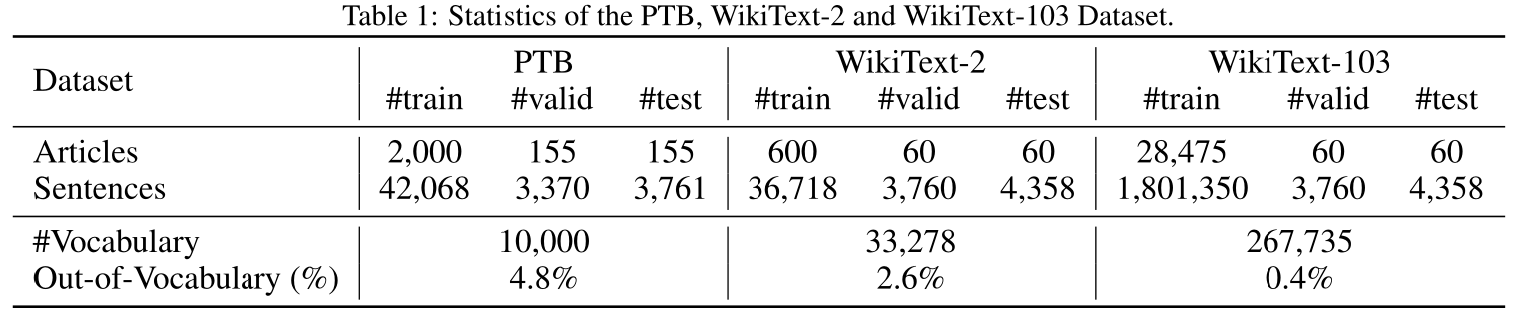
\includegraphics[scale=0.33]{data.png}
  \end{center}
\end{frame}
\begin{frame}[<+->]{Evaluation Metrics}
\begin{itemize}
  \item PPL:\begin{equation}\label{equ:ppl}
   \mathrm{PPL}(w_1,\cdots,w_T)=\sqrt[T]{\frac{1}{\prod_{t=1}^T p(w_t|w_{1:t-1})}}
\end{equation}

\item $\mathrm{WER}$ is the percentage of erroneously recognised words(deletions, insertions, substitutions) to the total number of words:
\begin{equation}\label{equ:wer}
  \mathrm{WER} = \frac{\text{Insertions + Deletions + Substitutions}}{\text{Actual~words~in~transcript}}
\end{equation}
\item REF: What a bright day

\item HYP: What a light day
\end{itemize}
\end{frame}

\begin{frame}[<+->]{Context Representation}

\begin{itemize}
  \item Feedforward Net: \begin{equation}h_t \leftarrow f(W\times E{[w_{t-n-1};\cdots,w_{t-1}]}  +b).\end{equation}
  \item Recurrent Net:\begin{equation}h_t \leftarrow RNN(W\times E(w_t) + U\times h_{t-1} +b).\end{equation}
  \item Convolution Net: \begin{equation}h_t \leftarrow RNN(W \times CNN(w_t) + U\times h_{t-1} +b).\end{equation}
\end{itemize}

\end{frame}


\begin{frame}[<+->]{Impact of the Recurrent Cells}
\begin{table}[!b]
\setlength{\abovecaptionskip}{0pt}
\setlength{\abovedisplayskip}{0pt}
\small
  \centering
  \caption{Recurrent cells on Wikitext-2 dataset.\label{tab:rnn}}
\begin{tabular}{lccc}
  \toprule
  \multirow{2}{*}{Recurrent Cells} & \multirow{2}{*}{Time(ms)}&Validation Set & Testing Set\\
  && PPL / WER & PPL / WER\\ \midrule
  1$\times$RNN Relu~\cite{DBLP:journals/jmlr/GutmannH10} &176.4&260.52 / 80.00\%&238.75 / 80.02\%\\
  1$\times$RNN Tanh~\cite{DBLP:journals/iclr/JiVSAD15}   &176.2&250.57 / 79.61\%&230.98 / 79.32\%\\
  1$\times$LSTM~\cite{7508408}                  &\textbf{189.5}&180.98 / 77.16\%&165.60 / 76.67\%\\
  1$\times$GRU~\cite{DBLP:journals/corr/ChungGCB14}      &191.3&\textbf{179.59 / 77.09\%}&\textbf{165.32 / 77.07\%}\\ \midrule
  2$\times$RNN Relu~\cite{DBLP:journals/jmlr/GutmannH10} &266.3&190.52 / 73.01\%&198.75 / 73.02\%\\
  2$\times$RNN Tanh~\cite{DBLP:journals/iclr/JiVSAD15}   &266.3&189.57 / 72.62\%&260.98 / 72.32\%\\
  2$\times$LSTM~\cite{7508408}                  &\textbf{279.4}&164.98 / 71.17\%&165.60 / 71.67\%\\
  2$\times$GRU~\cite{DBLP:journals/corr/ChungGCB14}      &281.2&\textbf{158.59 / 70.08\%}&\textbf{155.32 / 70.07\%}\\
  \bottomrule
\end{tabular}
\end{table}
\end{frame}


\begin{frame}[<+->]{Next-utterance Prediction}

\begin{figure}
\centering
\subfloat[RNNLM]{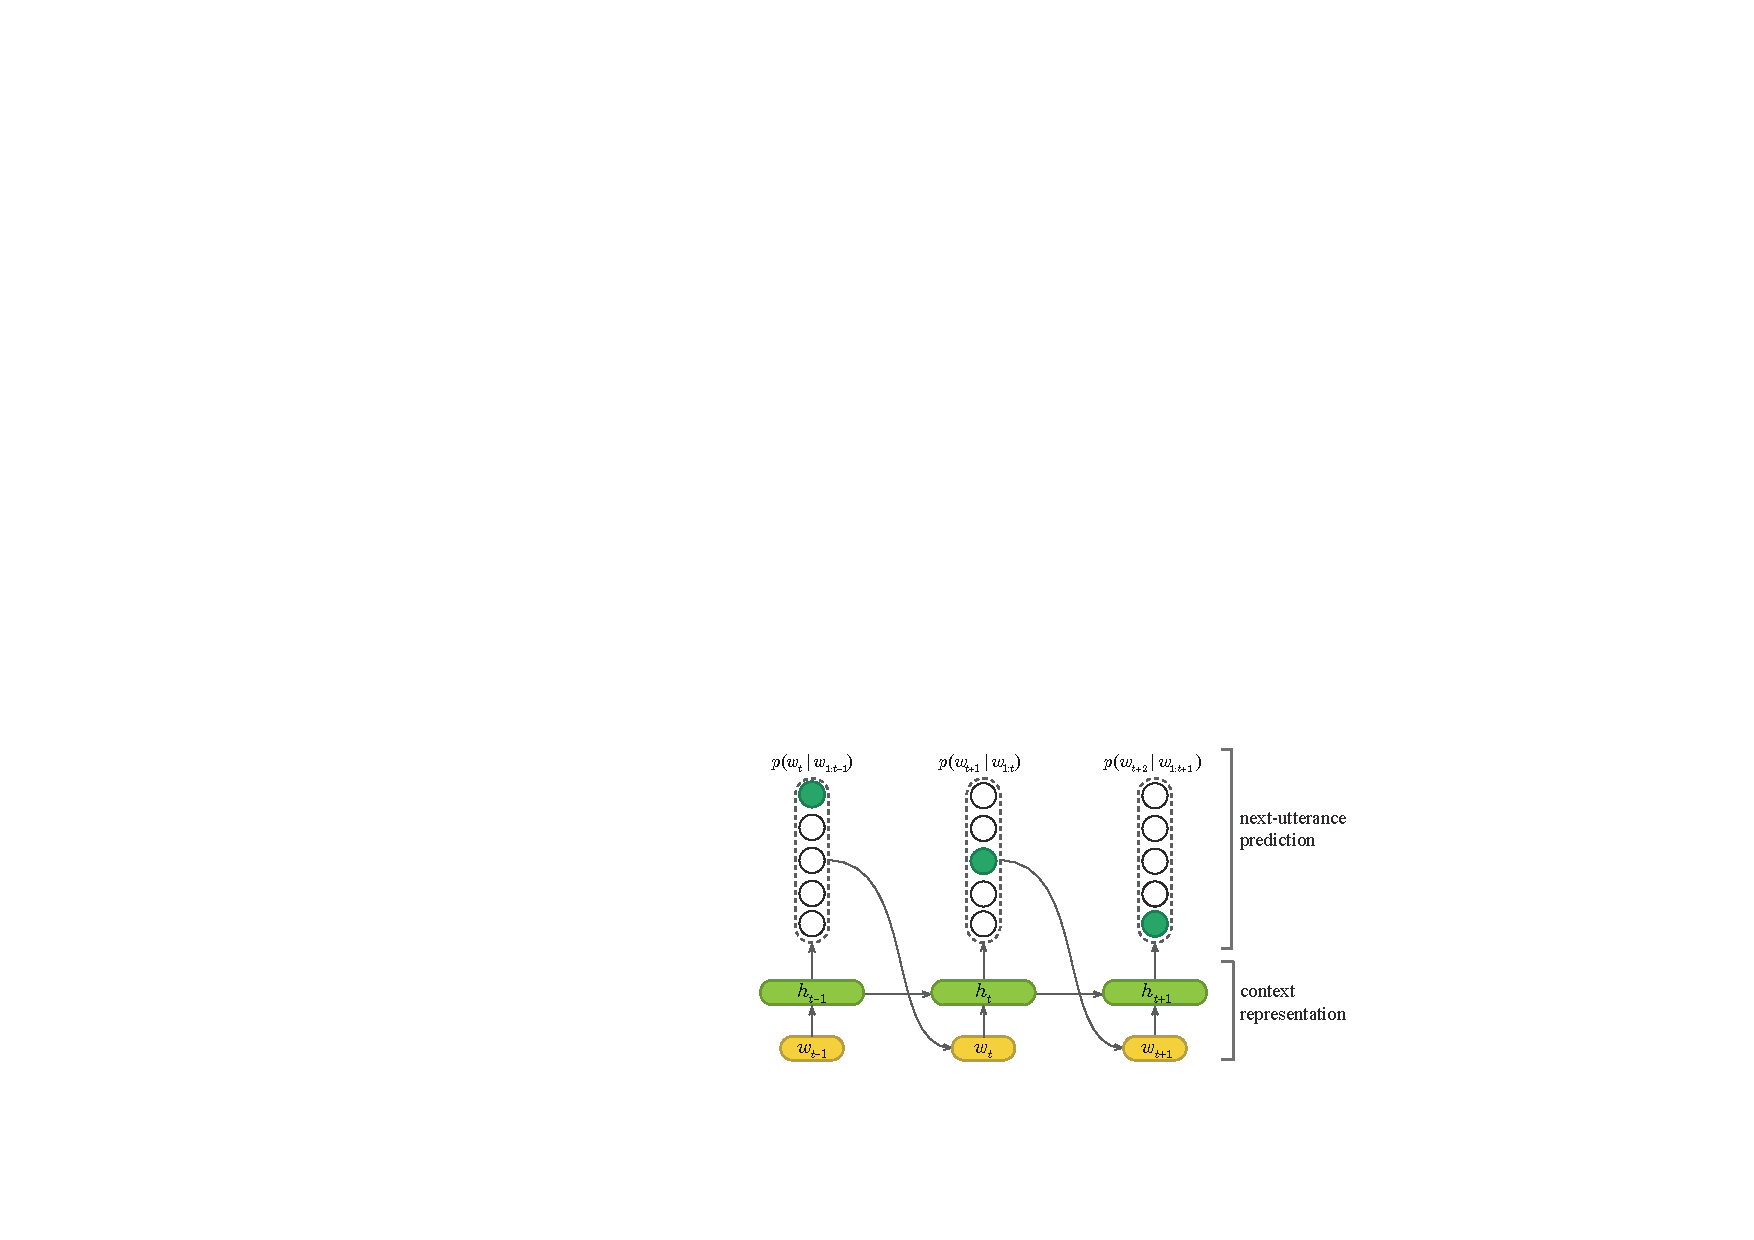
\includegraphics[scale=.45]{lm}}
~
\subfloat[vocab size 267,735]{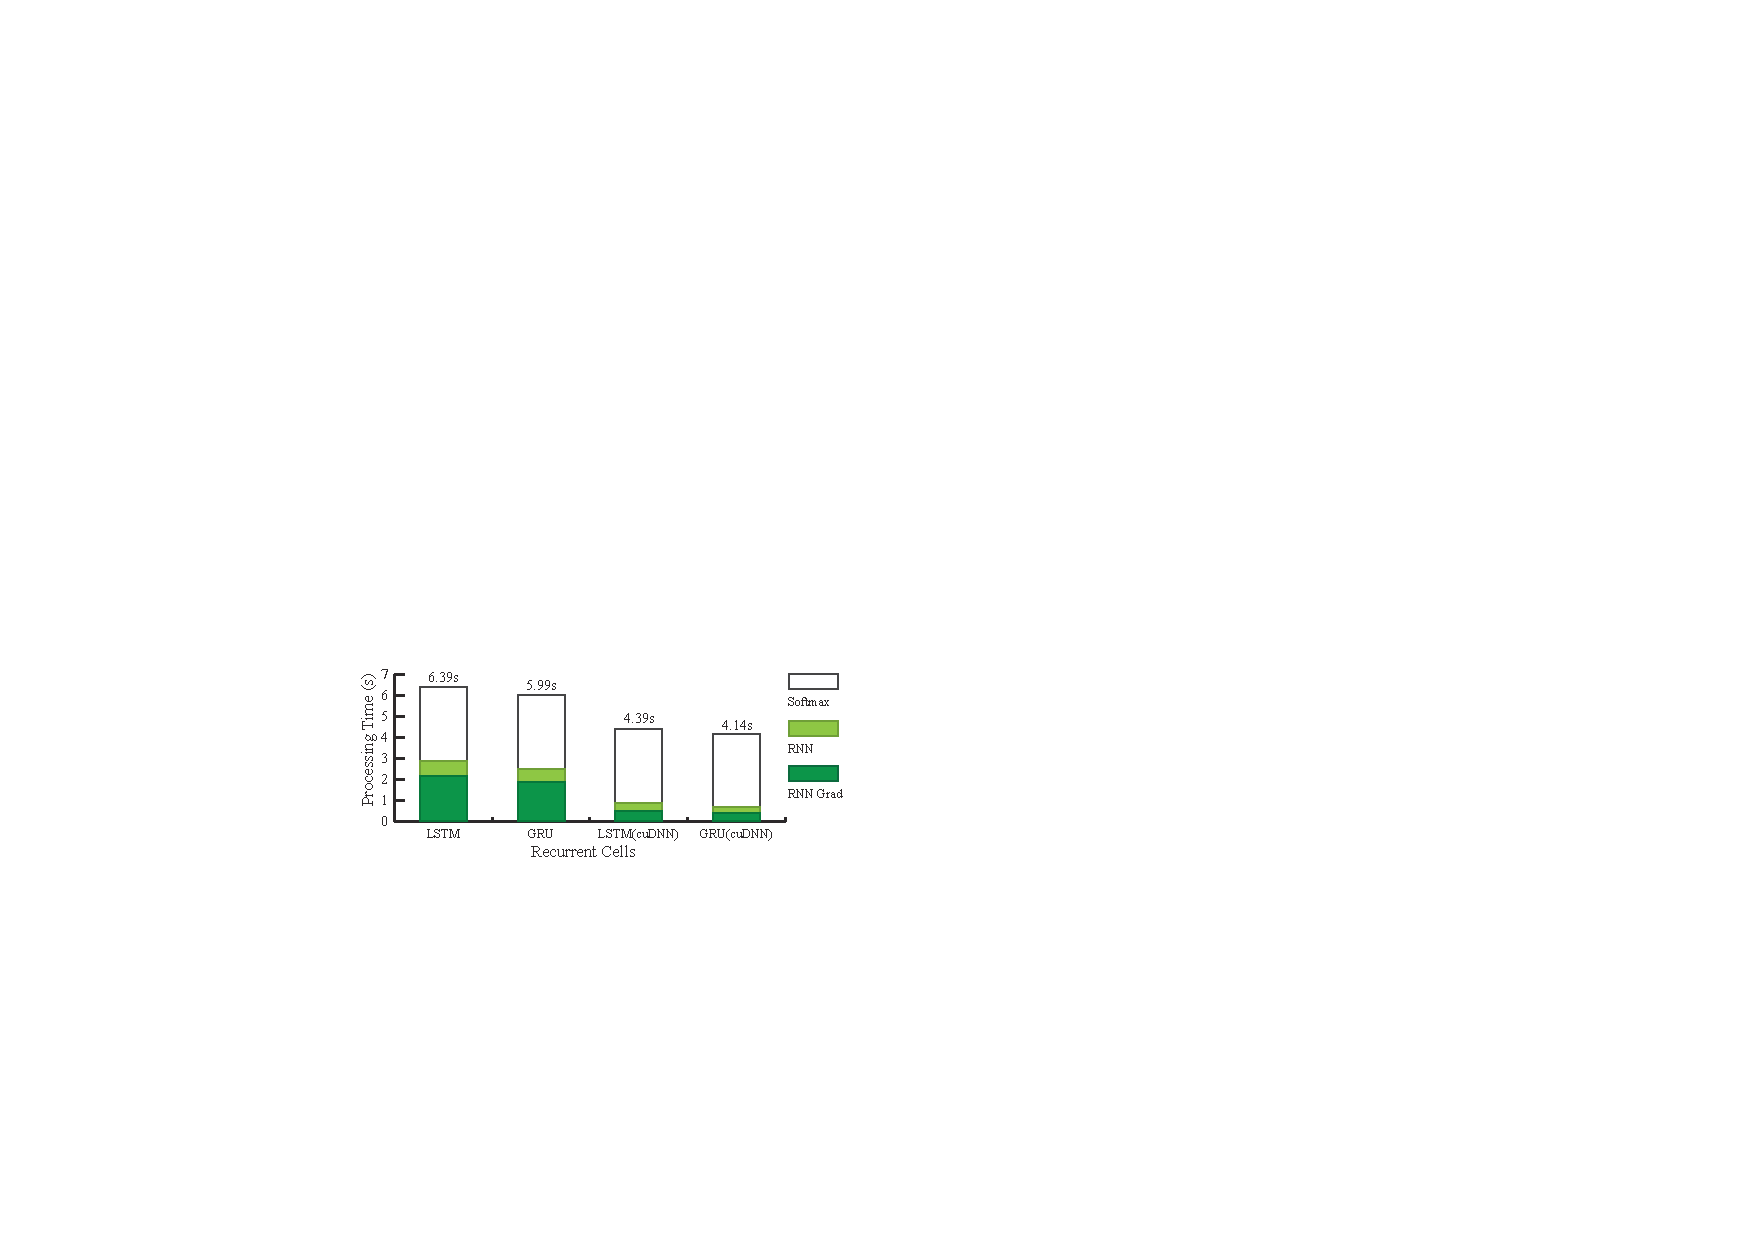
\includegraphics[scale=.7]{rnn_timing}}
\end{figure}

\begin{equation}
\log p(w_i|h) = \theta^w_i h-\log \sum_{w_j\in \mathcal{V}}{\exp(\theta^w_j h)}
\end{equation}
{How to ease the issue?}
\begin{itemize}
  \item Vocabulary truncation;
  \item Sampling-based approximation;
  \item Vocabulary Factorization.
\end{itemize}
\end{frame}

\begin{frame}[<+->]{Vocabulary Truncation}
\begin{itemize}
  \item word level: keep the top frequent words, the latter are dealt with n-gram model~\cite{DBLP:journals/csl/Schwenk07}.
  \item sub-word level: learned by byte-pair-encoding strategies~\cite{DBLP:conf/acl/SennrichHB16a,Gage:1994:NAD:177910.177914}.
  \begin{center}
    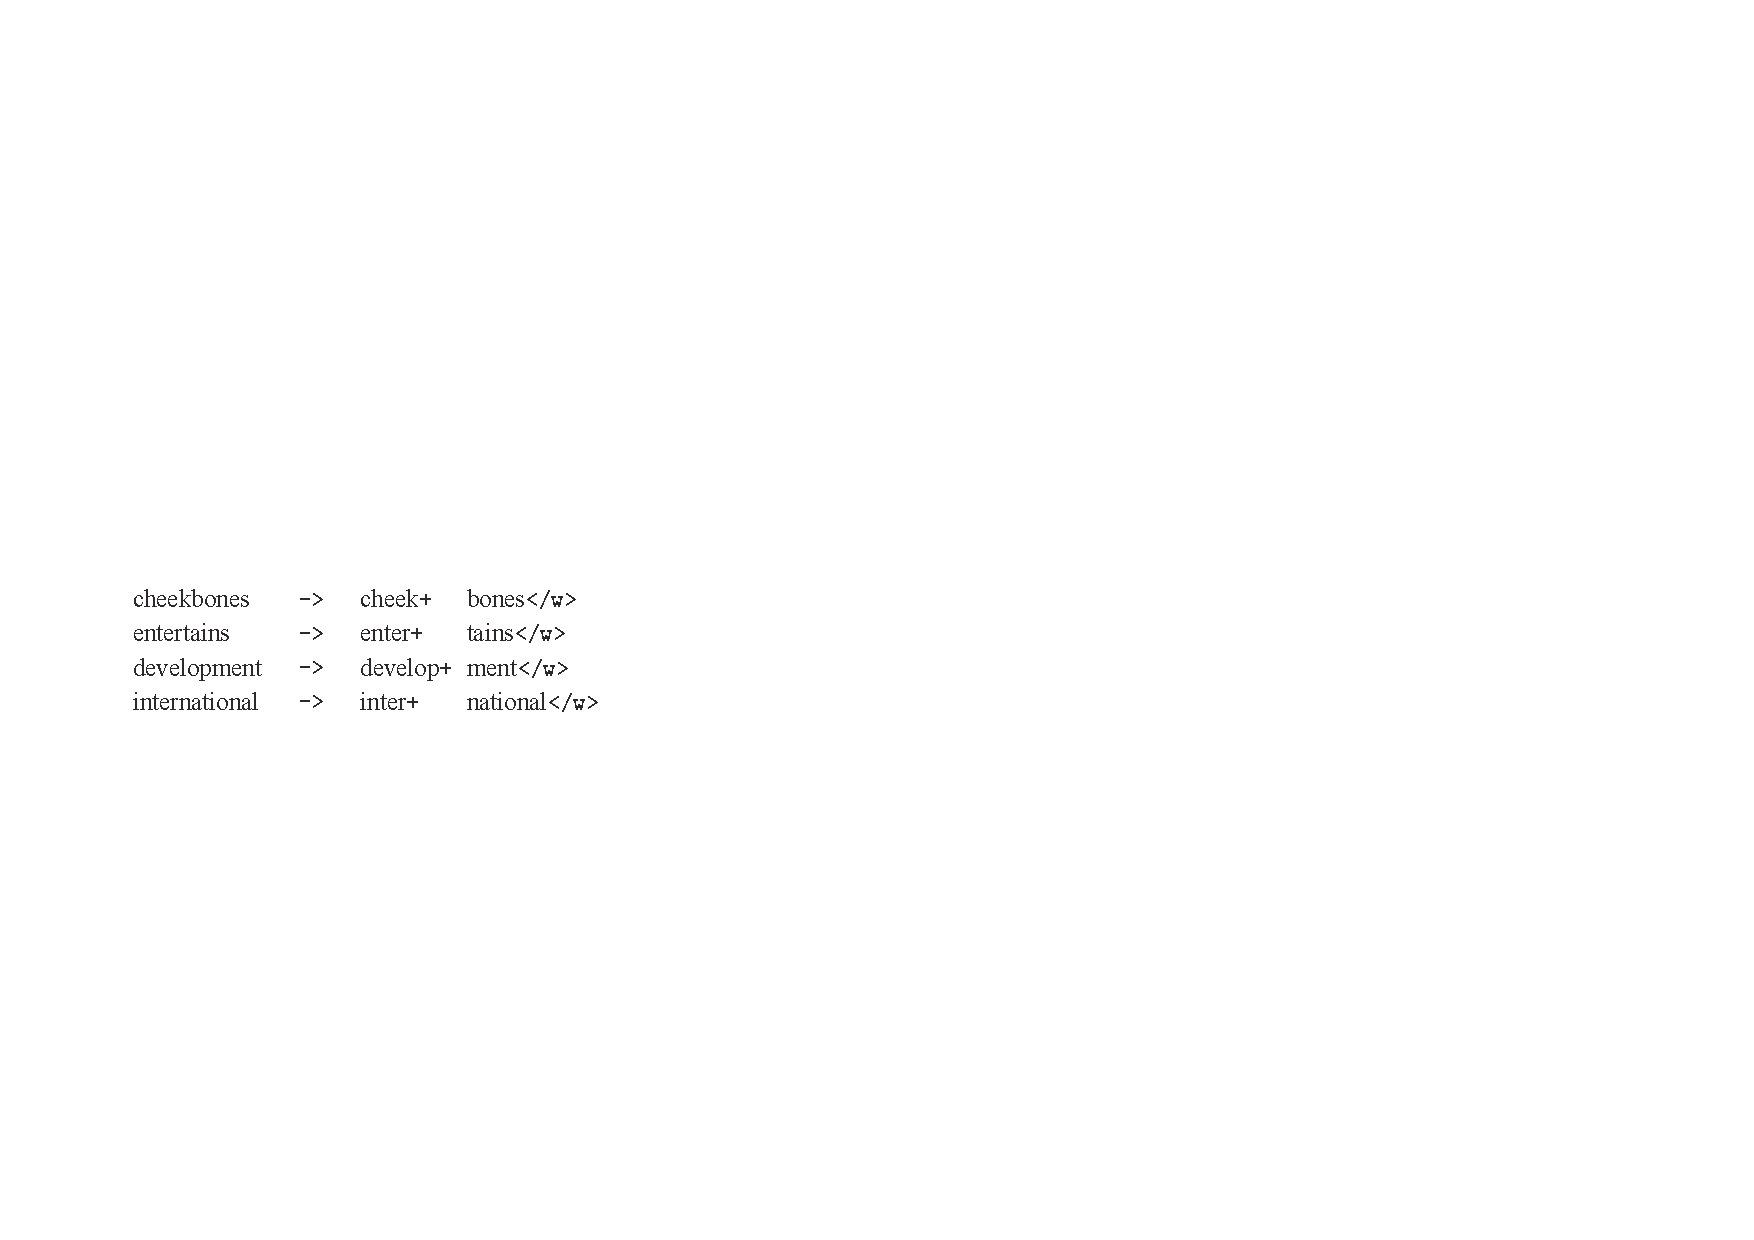
\includegraphics[scale=0.7]{subword}
  \end{center}
  \item Character-level: ``$a-zA-Z@~!\#$''~\cite{DBLP:journals/corr/JozefowiczVSSW16}.
\end{itemize}
\end{frame}

\begin{frame}[<+->]{Vocabulary Truncation}
Character level:  The input word are replaced by Convolution module with character.

  \begin{center}
    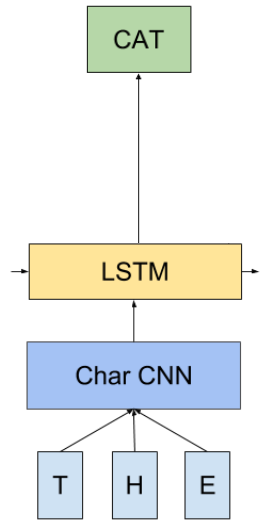
\includegraphics[scale=0.33]{lm1b_arch_a.png}
  \end{center}
\end{frame}

\begin{frame}[<+->]{Sampling based Approximation}
\begin{itemize}
\item {Possible ways:}
\begin{itemize}
  \item Importance sampling: the loss will not converge~\cite{DBLP:journals/tnn/BengioS08}.
  \item Noise contrastive estimation: good and simple~\cite{DBLP:conf/icml/MnihT12}.
  \item Blackout sampling: reasonable but results are vague~\cite{DBLP:journals/iclr/JiVSAD15}.
\end{itemize}
\item {Questions:}
\begin{itemize}
  \item how to select a suitable prior word distribution $p(w)$ to be sampled?
  \item how to sample with efficiency? alias methods~\cite{10.2307/2683739,DBLP:conf/emnlp/VaswaniZFC13}.
\end{itemize}
\end{itemize}
\end{frame}

\begin{frame}[<+->]{NCE \& Blackout}
NCE: the model learns to classify $w_0$ from $\{w_1\cdots w_k\}$, where $w_0$ is the empirical example and $\{w_1\cdots w_k\}$ are noise samples generated from a prior distribution $q(w)$.
\begin{equation}
\begin{split}
&p_n(w_i|h) = \frac{1}{K} \sum_{j\in S_K} \frac{q_j}{q_i} p_{\theta}(w_j |h),\\
&p_{\theta}(D = 1|w_i, h) = \frac{p_{\theta}(w_i|h)}{p_{\theta}(w_i|h) + Kp_n(w_i|h)}.
\end{split}
\end{equation}

Blackout:
\begin{equation}\label{equ:nce}
p_{\theta}(D = 1|w_i, h) = \frac{q_i \exp(\theta_i, h)}{q_i \exp(\theta_i, h) +\sum_{j\in S_K} q_j \exp(\theta_j, h)}.
\end{equation}
\end{frame}

\begin{frame}[<+->]{NCE \& Blackout}
\begin{figure}[t]
\setlength{\abovecaptionskip}{0pt}
\setlength{\belowcaptionskip}{0pt}
  \centering
  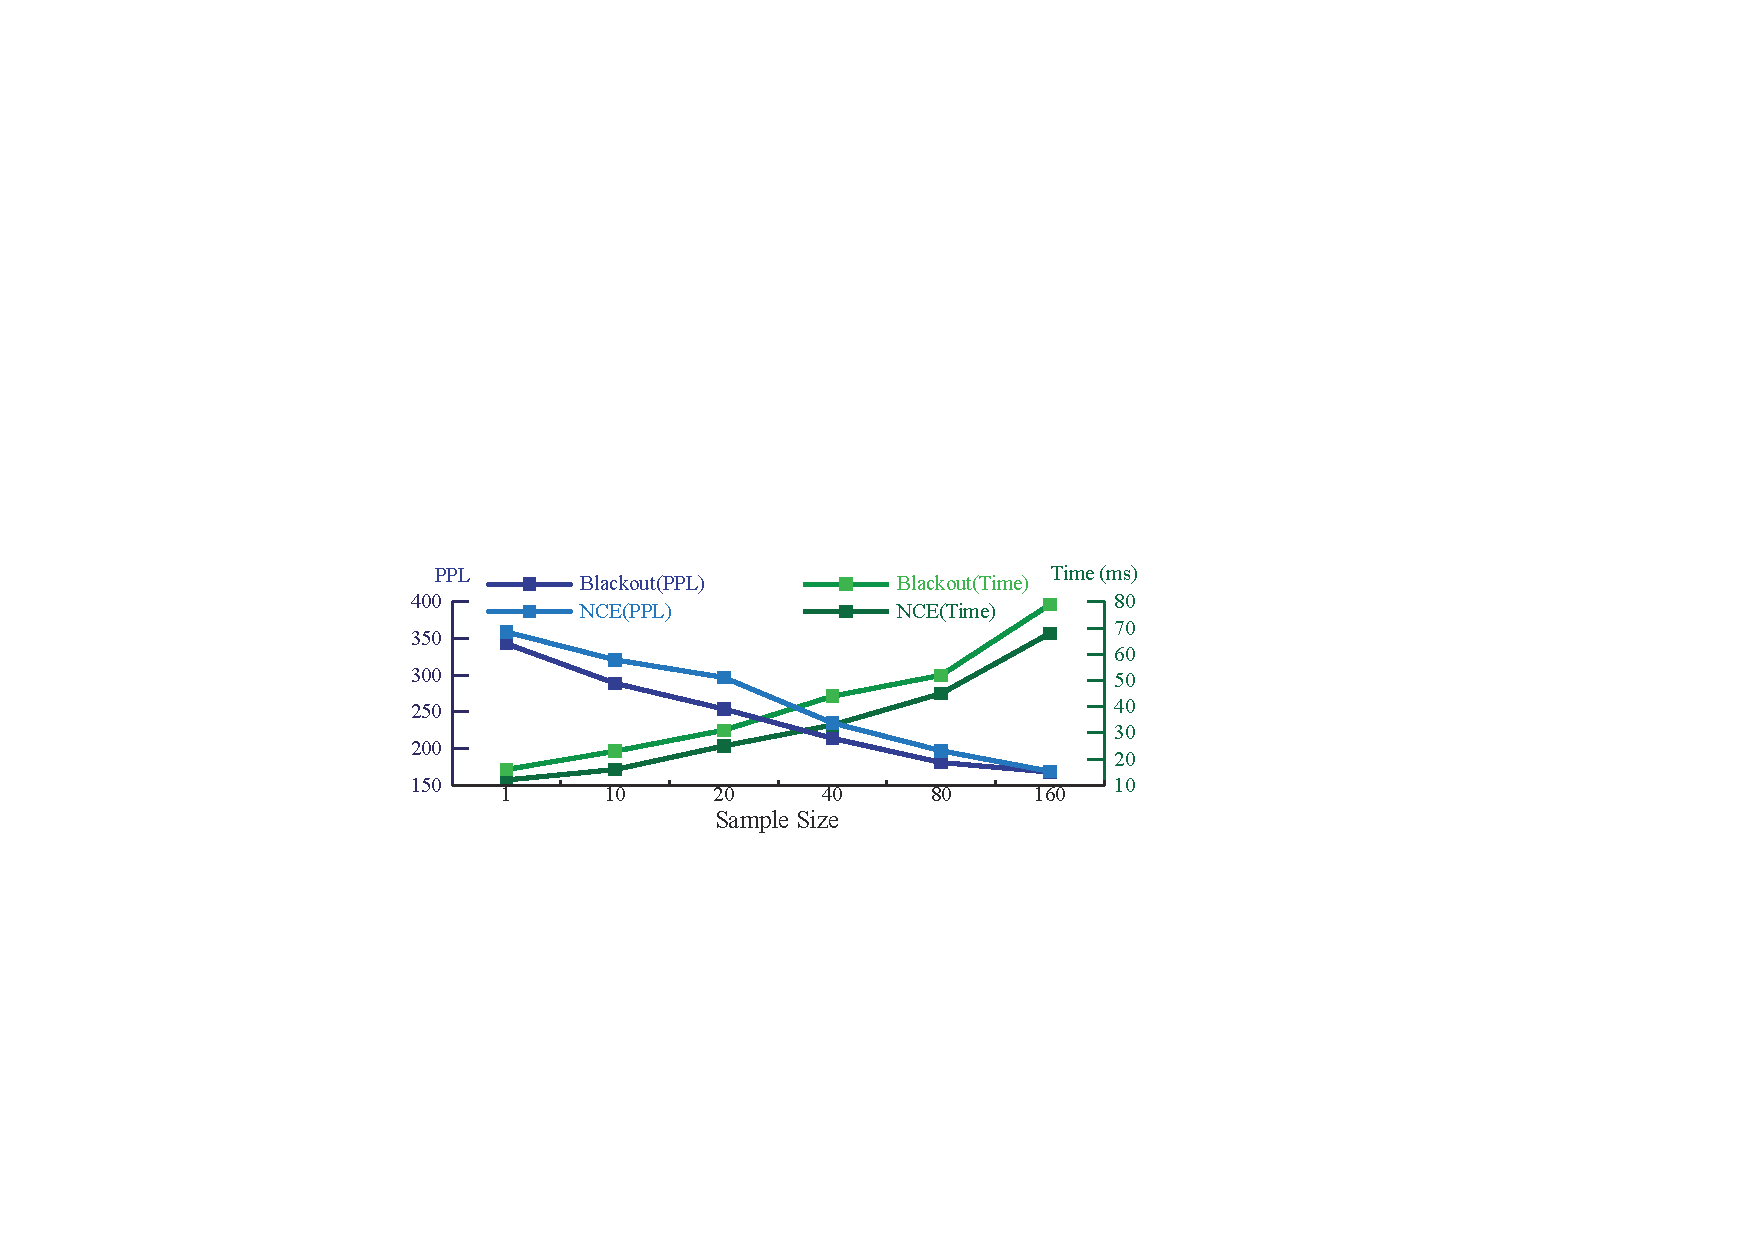
\includegraphics[width=0.85\columnwidth]{nce_blackout}
  \caption{Perplexity and time comparsion of different sample size with the NCE and Blackout methods on Wikitext-2 dataset.}\label{fig:blackout_nce}
\end{figure}
\end{frame}

\begin{frame}[<+->]{Vocabulary Factorization}

Class based hierarchical softmax.
  \begin{equation}
  \begin{split}
p(w|h)=&p^c(\mathcal{C}(w)|h)\cdot p^w(w|\mathcal{C}(w),h) \\
& w\in \mathcal{C}(w),\mathcal{V}=\bigcup _{i = 1}^\mathcal{C}{c_i} \\
&c_i \bigcap c_j=\phi, \text{If} i\ne j, \\
\end{split}
\end{equation}

  \begin{center}
    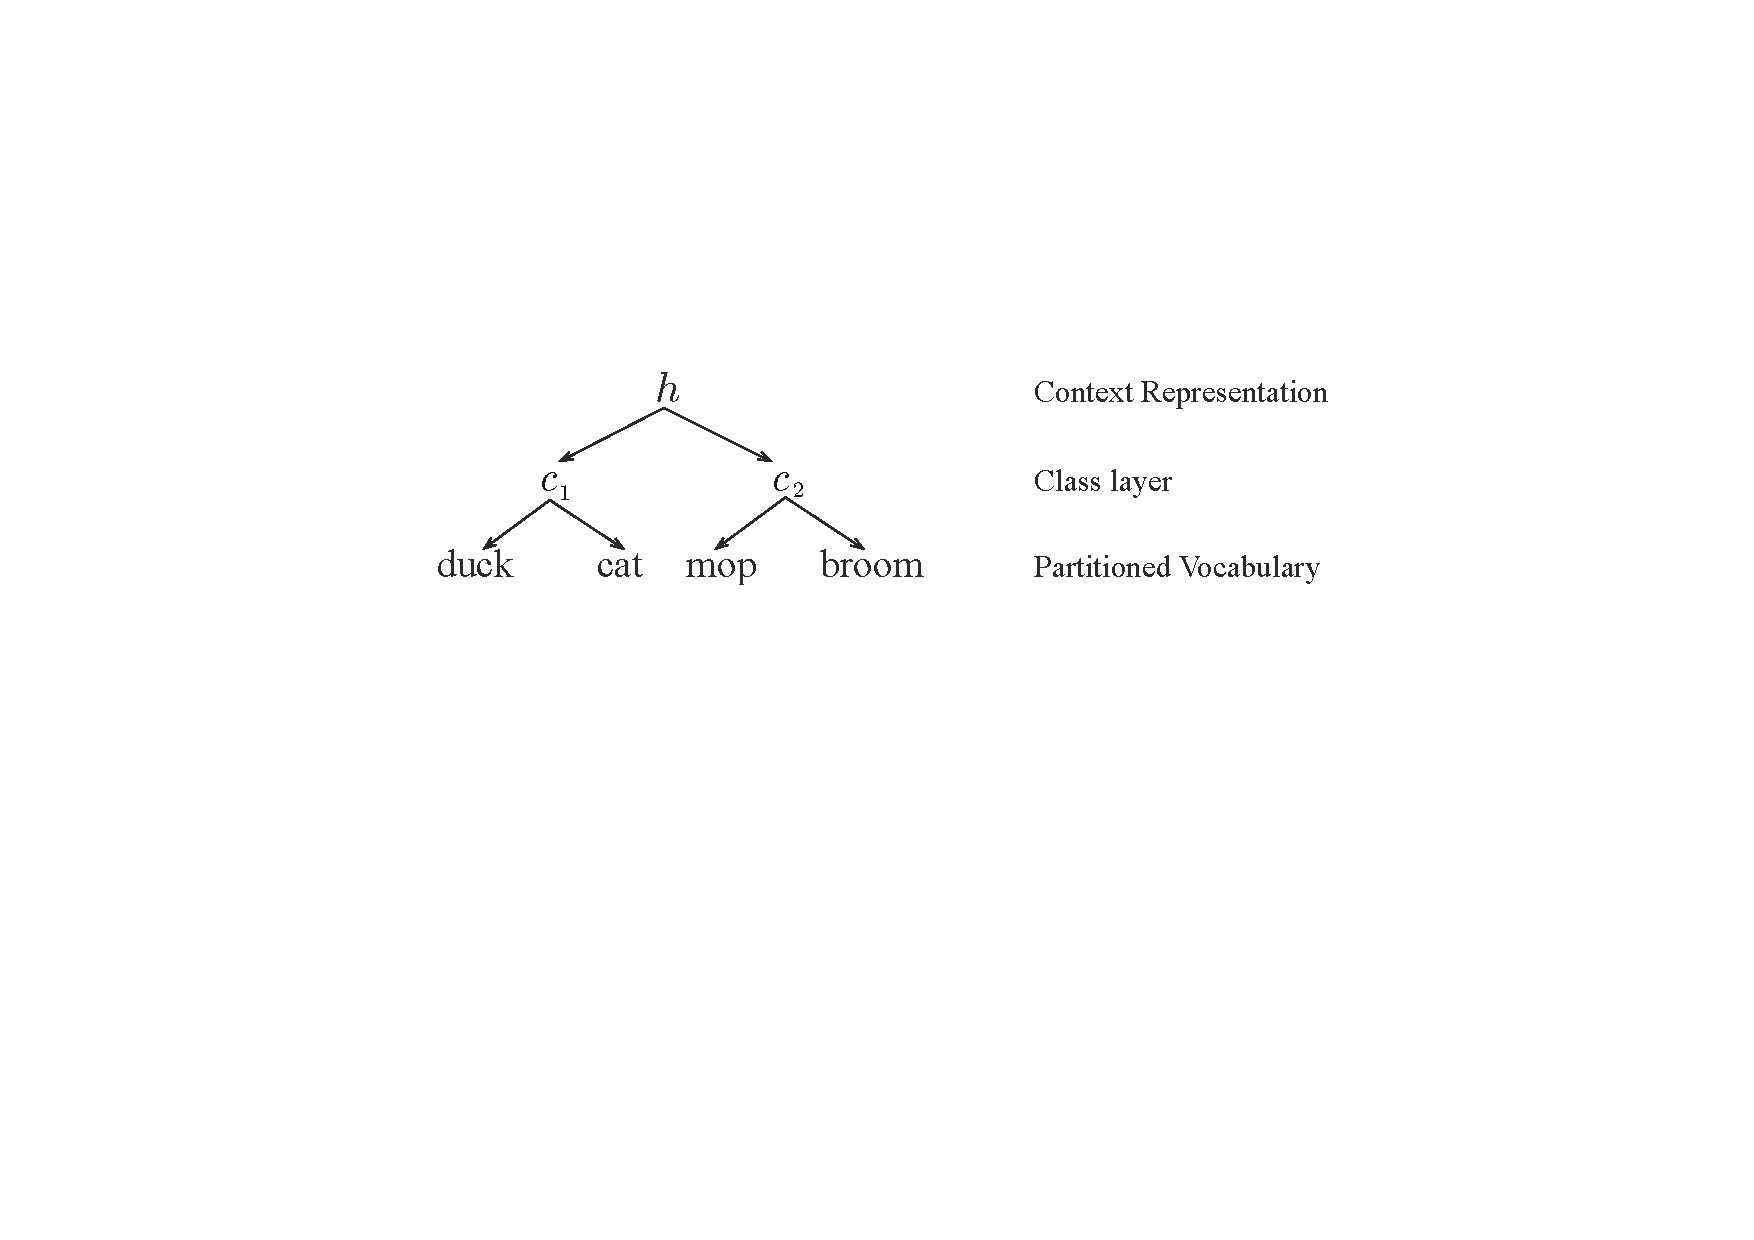
\includegraphics[scale=0.6]{case_chsm}
  \end{center}
\end{frame}

\begin{frame}[<+->]{Vocabulary Factorization}
\begin{table}
  \centering
  \caption{Perplexity and Word Error Rate of cHSM method on Wikitext-2 Dataset.\label{table:clustering}}
  \begin{tabular}{lccccc} \toprule
  &Branch& Epoches& PPL \& WER &Time(ms)\\\midrule
  &10/3330&193&211.51 / 77.41 &788\\
  &20/1664&252&220.01 / 77.71&549\\
  &40/832&273&236.56 / 77.95&302\\
  &80/417&291& 241.12 / 78.25&170\\
  &160/208&301&247.25 / 79.21&93\\
  &182/183&339&253.35 / 79.92&86\\
\bottomrule
\end{tabular}
\end{table}
\end{frame}

\begin{frame}[<+->]{Vocabulary Factorization}
Tree based hierarchical softmax.
\begin{center}
    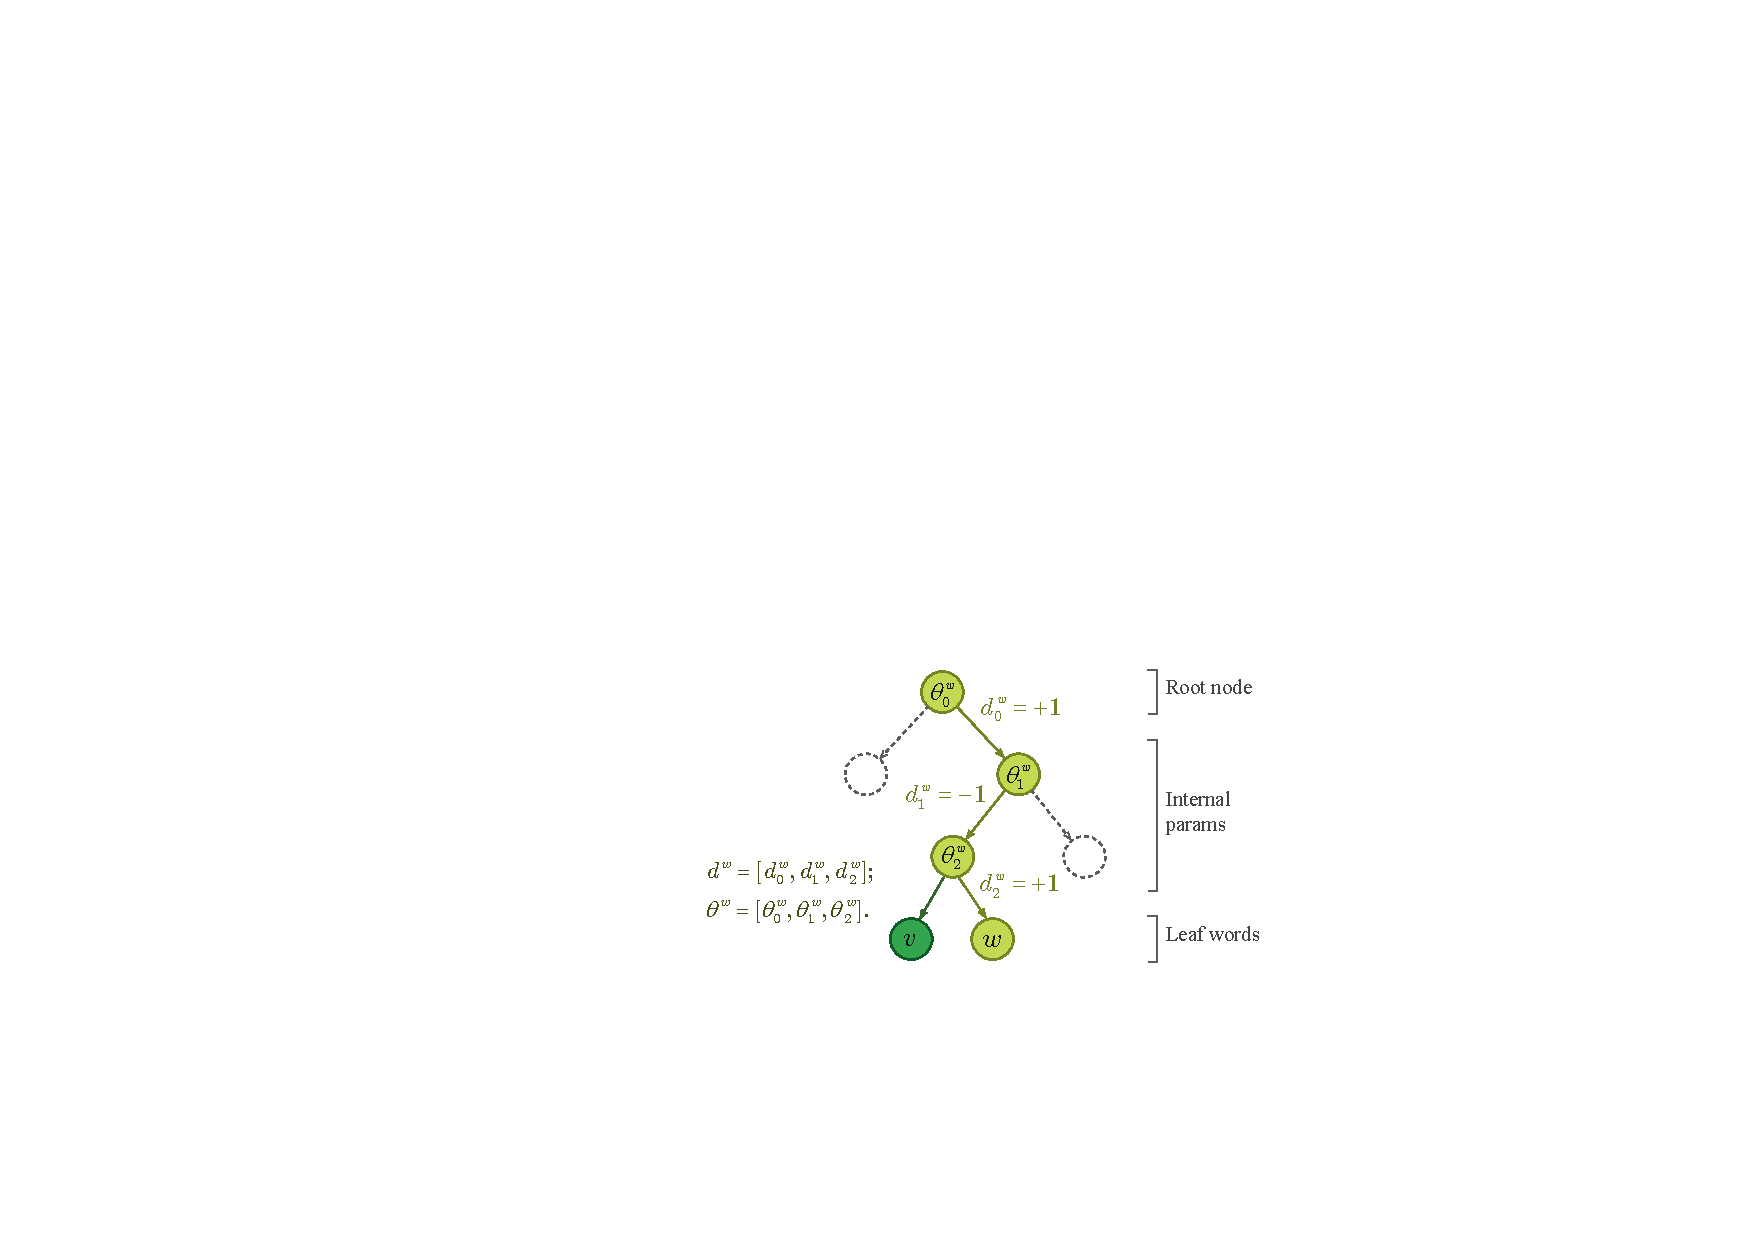
\includegraphics[scale=0.7]{thsm}
  \end{center}
\begin{itemize}
\item \begin{equation}
p(d^w_i|\theta_{i}^w,h) =\sigma(\theta_{i}^w h)^{d_i^w}\times[1-\sigma(\theta_{i}^w h)]^{1-{d_i^w}},d_i^w \in [0,1]
\end{equation}
  \item \begin{equation}
p(d^w_i|\theta_{i}^w,h) =\sigma(\theta_{i}^w h)^{d_i^w}, d_i^w \in [-1,1]
\end{equation}
  \item \begin{equation}
p(d^w_i=\pm 1|\theta_{i}^w,h) = \sigma({d_i^w}\theta_{i}^w h)
\end{equation}
\end{itemize}
\end{frame}

\begin{frame}[<+->]{Tree based Loss}
\begin{itemize}
  \item The probability of word $w$:
\begin{equation}\label{equ:pw}
\begin{split}
 \log p(w|h)=&\log\prod_{i=0}^{l^w-1} p(d^w_i|\theta_{i}^w,h) = \sum_{i=0}^{l^w -1} \log\sigma(d_i^w \theta_{i}^w h)\\
 =&\log\sigma({d^w}^\top \theta^w h)=\zeta(- {d^w}^\top \theta^w h )
 \end{split}
\end{equation}
\item  $\zeta(z)$ denotes the softplus function: $\zeta(z)= \log (1+\exp(z))$.
\item \begin{center}
    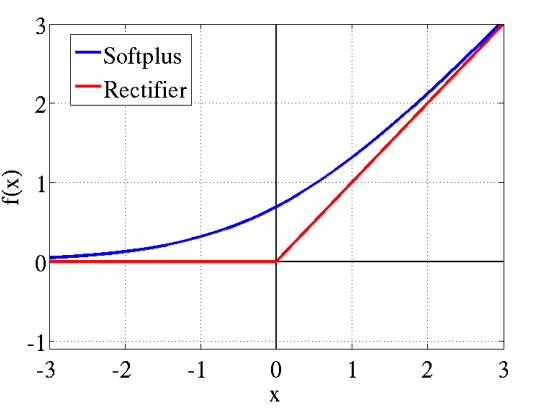
\includegraphics[scale=0.3]{softplus.png}
  \end{center}
\end{itemize}
\end{frame}


\begin{frame}[<+->]{Tree based Loss}
\begin{itemize}

\item The benefit:\begin{equation}
\sum_{w\in \mathcal{V}}{p(w|h)}=\sum_{w \in \mathcal{V}}\sum_{i=0}^{l^w-1}{\sigma(d_i^w\theta_{i}^w h)}=1.
\end{equation}
\end{itemize}
\end{frame}

\begin{frame}[<+->]{what did we optimise?}


\begin{itemize}
\item \begin{equation}
\begin{split}
   \mathcal{L}(\theta|h,w) =&  \zeta(- {d^w}^\top \theta^w h ) \\
   \mathcal{L'}(\theta|h,w) =&\sum_{i=0}^{l^w-1} \{(1-d'^w_i)\log (\sigma(\theta_{i}^w h))  + {d'^w_i}\log (1-\sigma (\theta_{i}^w h))\}
\end{split}
\end{equation}
  \item tHSM involves many tiny matrix multiplications, instead  we load all parameters $(d^w, \theta^w)$ directly as 1D vector and 2D matrix at the expense of runtime memory consumption and we consider the multiplications of this vector and giant matrix.
  \item A compact loss function of the model is deducted and the nodes' log-probability are calculated simultaneously which results in better time efficiency for p-tHSM model.
\end{itemize}
\end{frame}


\begin{frame}[<+->]{the performance}
\begin{figure}[!t]
\setlength{\abovecaptionskip}{0pt}
\setlength{\belowcaptionskip}{0pt}
  \centering
  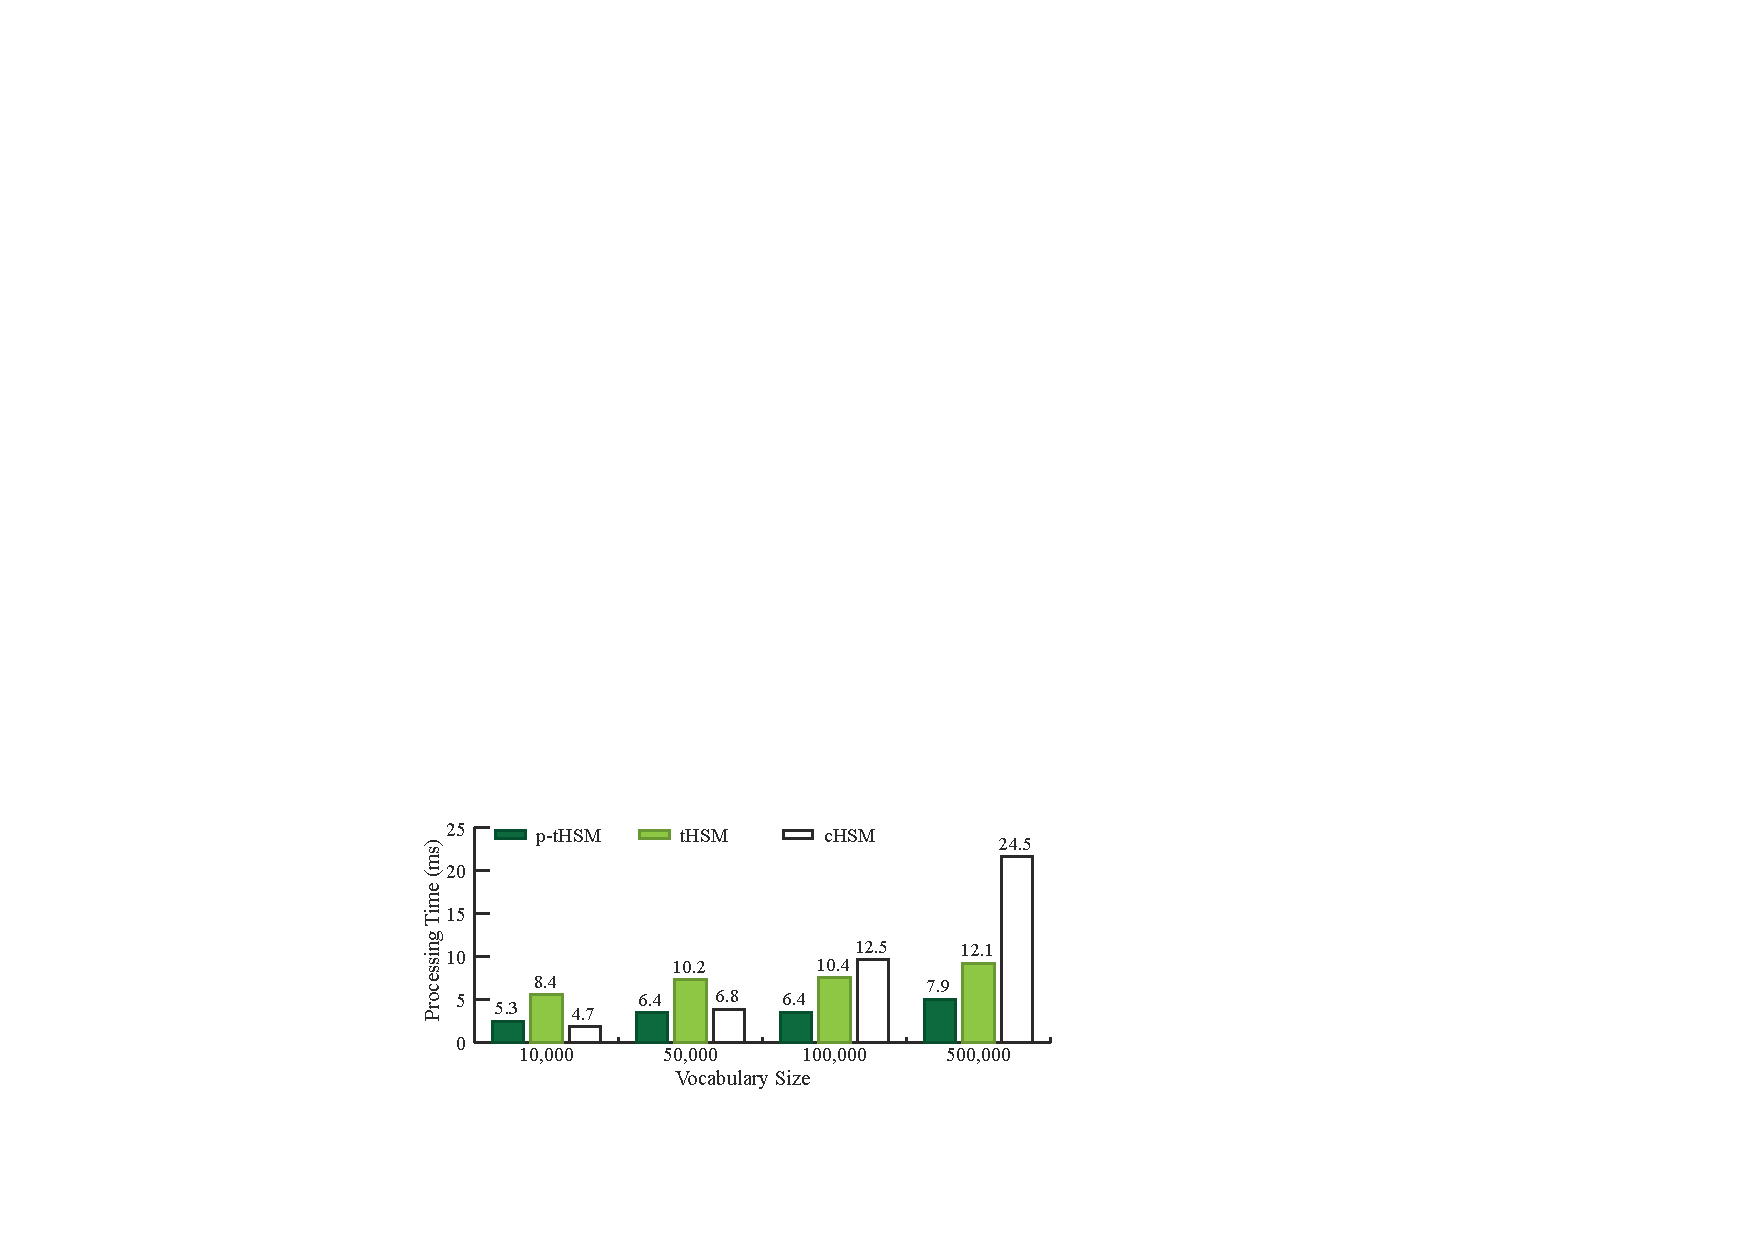
\includegraphics[width=0.95\columnwidth]{all_time}
  \caption{Scalability of cHSM, tHSM and p-tHSM algorithms with relevance to the vocabulary size.}\label{fig:hsm_benchmark}
\end{figure}
\end{frame}
\begin{frame}[<+->]{The performance}

\begin{table}[!t]
\setlength{\abovecaptionskip}{0pt}
\setlength{\abovedisplayskip}{0pt}
  \centering
  \caption{Runtime time and memory comparison on GPUs and CPUs with WikiText-103 Dataset.\label{tab:time}}
\begin{tabular}{lcrrrr}
  \toprule
   &Runtime &\multicolumn{2}{c}{Total Time(ms)} & \multicolumn{2}{c}{Forward Time(ms)}   \\
   \cmidrule(lr){3-4}  \cmidrule(lr){5-6}
	&Memory & CPU&GPU & CPU& GPU \\ \midrule
Softmax & $\mathcal{|HV|}$ &510.4  &262.1&352.2& 62.9 \\
cHSM    & $2\mathcal{|H|\sqrt{|V|}}$&506.5  &\textbf{40.6}&28.7&14.6 \\
tHSM    &$\mathcal{|H|}$&1,004.0 &444.4 & 8.1&  5.6   \\
p-tHSM  &$\mathcal{|H|\log{|V|}}$ &\textbf{383.5}&	86.4 &\textbf{7.0}&	\textbf{1.4} \\
  \bottomrule
\end{tabular}
\end{table}
\end{frame}

\begin{frame}[<+->]{Tree-based Inference}
\begin{itemize}
  \item getting the $\arg\max$ word under the given contexts: $\log p(w_t|h)$:
  \begin{equation}
\begin{split}
    p(w|h) =&\sigma({d^w}^\top \theta^w h)\\
   \log p(w|h) =& -\zeta(- {d^{w}}^\top \theta^{w} h )
\end{split}
\end{equation}
  \item searching for the most possible next-utterance words in the whole vocabulary.
  \begin{itemize}
  \item If $p(d^w_i |\theta_{i}^w,h) \ge 0.5$, go to the left child.
  \item Else, goto the right branch.
   \end{itemize}
\end{itemize}
\end{frame}




\begin{frame}[<+->]{The greedy algorithm}
\begin{table}[!t]
\setlength{\abovecaptionskip}{0pt}
\setlength{\abovedisplayskip}{0pt}
  \centering
  \caption{Word error rate with different searching rules on Wikitext-2 dataset.\label{tab:search}}
\begin{tabular}{llccc}
  \toprule
   & Type&Time(ms)&Valid set & Test set \\ \midrule
  \multirow{2}{*}{p-tHSM}                  &global&161& \textbf{76.67\%}&\textbf{75.35\%}\\
        &greedy&\textbf{30} & 79.61\%&79.32\%\\
  \bottomrule
\end{tabular}
\end{table}
\end{frame}


\begin{frame}[<+->]{Init of words over tree}
\begin{itemize}
  \item Unigram clustering (Huffman clustering)
  \item Bigram clustering (Brown clustering)
  \item Semantic clustering (cluster with word embedding)
\end{itemize}

\begin{table}[!t]
\setlength{\abovecaptionskip}{0pt}
\setlength{\abovedisplayskip}{0pt}
  \centering
   \caption{Perplexity of p-HSM algorithms with various clustering methods on Wikitext-2 Dataset.\label{table:p-thsm}}
  \begin{tabular}{lcccc} \toprule
  Methods   &Construction&Max Tree Depth &Valid & Test   \\ \midrule
  Uigram  &3min&12 &218.42& 216.05     \\
  Bigram  &35h&21& 186.23& 189.58\\
  Semantic &26h &18& \textbf{163.12} & \textbf{178.78}\\
\bottomrule
  \end{tabular}
\end{table}
\end{frame}

\begin{frame}[<+->]{Overall Performance}
small dataset: use the softmax.

large dataset: use the optimization.
\begin{center}
    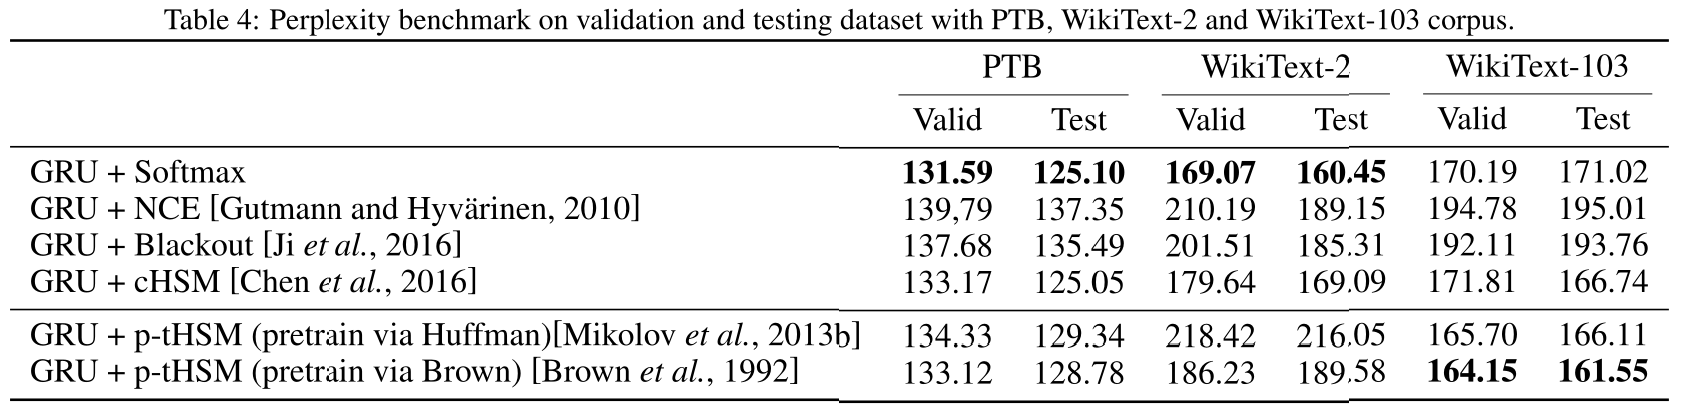
\includegraphics[scale=0.33]{benchmark.png}
  \end{center}
\end{frame}


\begin{frame}[<+->]{Summary}
\begin{itemize}
\item Knowledge on recurrent language model;
\item Reviews on historical optimization methods;
\item Introduce our work on hierarchical softmax;
\item Experimental results.
\end{itemize}
\end{frame}
\begin{frame}[<+->]{Thanks}
\begin{itemize}
\item Release: https://github.com/jiangnanhugo/lmkit;
\item Question ?
\end{itemize}
\end{frame}
\bibliographystyle{alpha}
\bibliography{reference}
\end{document}
